\section{Introduction}
\label{sec:intro}

\begin{figure}[t]
  \centering
  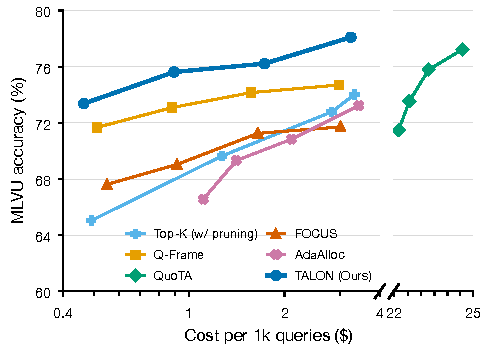
\includegraphics[width=\linewidth]{fig/budget_curve.pdf}
  \caption{\textbf{Accuracy against cost on MLVU} (Qwen3-VL-8B). Each line traces one method across token budgets
    from 1,536 to 12,288. Cost prices the input tokens of 1,000 queries at OpenRouter rates. The scorer calls of QuoTA place it beyond the axis break.}
  \label{fig:budget}
\end{figure}

Vision-language models (VLMs) now answer open-ended questions about
videos~\cite{bai2025qwen3vl,wang2025internvl35}, and the videos of practical interest are long. Applications such as
video analytics over camera feeds~\cite{yan2025ava} and search over lectures, meetings, and broadcasts pose questions whose evidence occupies a few seconds of a video that
lasts from minutes to hours~\cite{fu2024videomme,zhou2024mlvu,wu2024longvideobench}.

Processing every frame of such a video is impractical: an hour of video at one frame per second yields millions of
visual tokens, far beyond the context window of current VLMs.
Existing systems, therefore, widely resort to retrieval-augmented generation (RAG). They index the video offline,
either by embedding its frames and transcript~\cite{luo2024videorag,jeong2025videorag} or by building a graph over
its clips and entities~\cite{ren2025videorag,shen2025vgent,yan2025ava,yang2026g2frag,chen2026memdreamer,yan2026ecrag}, and supply the VLM with only the evidence
retrieved for each query.

Both forms of RAG, however, have limitations. Graph-based RAG attains high accuracy, but must caption and link
the whole video before the first question arrives, a cost that is often wasted because users query a video
sporadically. Embedding-based RAG is lightweight, but it operates at the frame level: it admits the top-$K$ frames
and passes each of them to the VLM at the same token cost. This uniform cost is wasteful, since the relevance of the
retrieved frames is highly uneven, and the value of a frame saturates with its token count (\cref{fig:value}), so
that most tokens of a frame are better spent on other frames. Token
compression~\cite{chen2024fastv,yang2024visionzip,shen2024longvu} mitigates this issue, but compresses every frame
independently, and recent query-aware methods vary the token count of frames only with fixed rules, such as
resolution tiers~\cite{zhang2025qframe} or shares proportional to relevance~\cite{luo2025quota}. None of these
methods solves for the division of a global token budget across frames, although a different division could reveal
useful evidence in other frames.

These limitations motivate us to move video RAG from frames to tokens. We present \name, a plug-and-play
\textbf{T}oken \textbf{AL}locati\textbf{ON} framework that is placed between a retriever and a VLM, and decides how
many tokens each retrieved frame and transcript segment receives. \name formulates this decision as one optimization
problem, which maximizes the relevance-weighted value of the evidence subject to a token budget.

Realizing this formulation raises two challenges. The first is to value tokens and to solve the allocation
efficiently. The Token Scheduler of \name learns a \textit{token value} function offline, discounts frames that
duplicate others already shown, and lets frames and transcript segments compete for the same budget. It solves the
resulting problem by iterative water-filling, and we derive the optimal allocation, which the
allocation rules of prior work do not attain. The second challenge arises in multi-turn conversations, where re-allocating tokens
for every question invalidates the KV cache that LLM serving systems reuse across
turns~\cite{kwon2023vllm,zheng2024sglang}. \name instead carries the allocation across turns: it updates the
relevance of cached frames with the attention of the VLM, and prefills only the tokens that the cache lacks, so that
the cumulative prefill of evidence tokens provably stays bounded.

We evaluate \name on MLVU, LongVideoBench, and Video-MME with two VLMs, and on the multi-turn MT-Video-Bench. At the
same budget of 12,288 tokens, \name improves the accuracy of Qwen3-VL-8B by 2.2 to 4.2 points over retrieval with
uniform token pruning, and matches or exceeds QuoTA, the strongest baseline, which requires 2.8--3.4$\times$ more
compute. With a quarter of the budget, \name is more accurate on MLVU than Q-Frame, FOCUS, and AdaAlloc at the full
budget (\cref{fig:budget}), and its gains carry over to graph-based retrieval when paired with VideoRAG. In
conversations, it uses up to 5.2$\times$ less compute at comparable accuracy.

Our contributions are as follows:
\begin{itemize}
  \item We introduce \name, a plug-and-play framework that formulates video RAG as one budgeted token allocation
    over frames and transcript segments.
  \item We design the Token Scheduler, which combines a learned token value with iterative water-filling, and derive
    the optimal allocation of its objective, which the allocation rules of prior work do not attain.
  \item We extend token allocation to multi-turn conversations with KV-cache reuse and attention-updated
    relevance, and prove that the cumulative prefill of evidence tokens stays bounded.
\end{itemize}
